% This is LLNCS.DEM the demonstration file of
% the LaTeX macro package from Springer-Verlag
% for Lecture Notes in Computer Science, version 1.1
\documentclass{llncs}
%

\usepackage[utf8]{inputenc} % accents
\usepackage{latexsym}
\usepackage{bbm}              % fontes doubles (pour les ensembles, par ex.)
\usepackage{graphicx}         % pour d'eventuelles figures
\usepackage{epsfig}           % (preferer graphicx, si possible)
\usepackage{amsmath}          % AMSTEX
\usepackage{amsfonts}
\usepackage{fancyhdr}
\usepackage{subfigure}




\usepackage{algorithm}
\usepackage{algorithmic}

\begin{document}

\title{Sparsification on Parallel Spectral Clustering
\thanks{This work was performed using HPC resources from CALMIP (Grant 2012-p0989)}}

\author{Sandrine Mouysset\inst{1} and Ronan Guivarch\inst{2}}

\institute{University of Toulouse, IRIT-UPS, France
\and
University of Toulouse, INP(ENSEEIHT)-IRIT, France}

\maketitle

\begin{abstract}
Spectral clustering is one of the most relevant unsupervised method able to
gather data without a priori information on shapes or locality. A parallel
strategy based on domain decomposition with overlapping interface is
reminded. By investigating  sparsification techniques and introducing sparse
structures, this parallel method is  adapted to treat very large data set in
fields of Pattern Recognition and Image Segmentation.
\end{abstract}
%
\section{Introduction}

Spectral clustering selects dominant eigenvectors of a parametrized affinity
matrix in order to build a low-dimensional data space wherein data points are
grouped into clusters \cite{speC}. This method based on eigendecomposition of affinity matrix is used in Pattern Recognition or  image segmentation  to cluster non-convex domains without a priori on the shapes. 
The main difficulties of this method could be
summarized by
the two following questions: how to automatically separate clusters one from
the other and how to perform clustering on large dataset, for example on image
segmentation. This means that we look for some full-unsupervising process with
parallelization.
Several studies exist for defining a parallel implementation which exploits linear
algebra \cite{song}, \cite{fowlkes} for the affinity computation of the whole data set
\cite{Chen10}. But the input parameters which are the affinity parameter and
the number of clusters limit these methods.
To address this limitation, a fully unsupervised parallel strategy based on
domain decomposition was proposed in \cite{mouysset3} which preserves the
quality of global partition thanks to overlapping interface. From the first
results, we have observed that the main part of the time is spent in the
spectral clustering step and we encountered memory limitation with large
problems.

In this paper, we study the robustness of the parallel spectral clustering with overlapping interface presented in  \cite{mouysset3} by
investigating sparsification techniques and introducing sparse structures and
adapted eigensolvers in order to treat larger problems. Then we test this improvements on geometrical examples and image segmentations.


\section{Parallel Spectral Clustering}
%

Let consider a data set $S=\{x_i\}_{i=1..n}\in \mathbb{R}^p$. Assume that the
number of targeted clusters $k$ is known. First, the spectral clustering
consists in constructing the affinity matrix based on the Gaussian affinity
measure between points of the dataset $S$.
After a normalization step, the $k$ largest eigenvectors are extracted. So
every data point $x_i$ is plotted in a spectral embedding space of
$\mathbb{R}^k$ and the clustering is made in this space by applying $K-means$
method. Finally, thanks to an equivalence relation, the final partition of
data set is defined from the clustering in the embedded space. Algorithm 1
presents the different steps of spectral clustering.
\begin{algorithm}
\caption{Spectral Clustering Algorithm}
%\begin{algorithmic}[1]
%\begin{algorithm}
Input: data set $S$, number of clusters $k$
\begin{enumerate}
\item Form the affinity matrix $A\in\mathbb{R}^{n\times n}$ defined by:
\begin{equation}
A_{ij}=\begin{cases}
\exp\left(-\frac{\left\|x_i-x_j\right\|^2}{(\sigma/2)^2}\right) \text{\  if $i\neq j$,}\\ \label{defaff}
0 \ \text{otherwise,}
\end{cases}
\end{equation}
\item Construct the normalized matrix: $L=D^{-1/2}AD^{-1/2}$ with $D_{i,i}=\sum_{j=1}^n A_{ij}$,
\item Assemble the matrix $X=[X_1X_2..X_k]\in \mathbb{R}^{n\times k}$ by stacking the eigenvectors associated with the {$k$} largest eigenvalues of $L$,
\item Form the matrix Y by normalizing each row in the $n \times k$ matrix X,
\item Treat each row of Y as a point in $\mathbb{R}^{k}$, and group them in $k$ clusters via the {\it K-means} method,
\item Assign the original point $x_i$ to cluster $j$ when row $i$ of matrix Y belongs to cluster~$j$. 
\end{enumerate}
\label{algo}
%\end{algorithmic}
\end{algorithm}


This spectral clustering method could be adapted for parallel implementation \cite{mouysset3} as a fully unsupervised method (see Figure \ref{parallel}). This avoid extracting the largest eigenvectors of a fully affinity matrix which complexity is of $O(n^3)$ \cite{yan2009fast}.
 
\begin{figure}
  \begin{center}
  {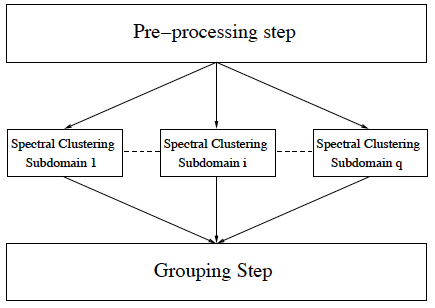
\includegraphics[width=0.6\linewidth]{Images/intersectionq}}
\end{center}
\caption{Principle of the parallel spectral clustering}
\label{parallel}
\end{figure}
The principle is based on domain decomposition with overlaps. 
By dividing the data set $S$ in $q$ sub-domains, each processor applies
independently the spectral clustering algorithm on the subsets and provide a
local partition. For each subdomain, a quality measure which exploits the
block structure of indexed affinity matrix per cluster is used to determine
the number of clusters. This heuristic avoids us to fix the targeted of clusters $k$. The final number of clusters $k$ will be provided after the grouping step.  
The gathering step is dedicated to link the local partitions from the sub-domains thanks to the overlapping interface and the following 
 transitive relation: $\forall x_{i_1}, x_{i_2}, x_{i_3} \in S,$
\begin{equation}
\text{if } \ x_{i_1},x_{i_2} \in C^1  \text{ and }  x_{i_2}, x_{i_3} \in C^2 \text{ then } C^1 \cup C^2 = P \text{ and } x_{i_1},x_{i_2}, x_{i_3} \in P \label{reltrans}
\end{equation}
where $S$ is a data set, $C^1$ and $C^2$ two distinct clusters and $P$ a larger cluster which includes both $C^1$ and $C^2$. 
By applying this transitive relation (\ref{reltrans})  on the overlapping interface, the connection between subsets of data is established and provides a
global partition.
%\pagebreak[4]
We can summarize this Master-Slave implementation with Algorithm 2 and Algorithm 3.
\begin{algorithm}
\caption{Parallel Algorithm: Master}
\label{algo-master}
\begin{algorithmic}[1]
%\begin{algorithm}
  \STATE Pre-processing step\\
        1.1 Read the global data and the parameters\\
        1.2 Split the data into $q$ subsets\\
        1.3 \begin{tabular}[t]{l}
            Compute the affinity parameter $\sigma$ with the formula given 
            in paper \cite{mouysset3}; \\
            the bandwidth of the overlapping is fixed to
            $3\times \sigma$ 
            \end{tabular}
  \STATE Send the sigma value and the data subsets to the other processors
         (\textsc{Mpi\_Send})
  \STATE Perform the Spectral Clustering Algorithm on its subset\\
         3.1 \begin{tabular}[t]{l}
             Computation of the spectrum of the affinity matrix
             (\ref{defaff}):
             classical routines \\
             from LAPACK library \cite{anderson1999lapack}
             are used to compute selected eigenvalues,\\
             eigenvectors of the normalized  affinity matrix $A$ for its
             subset of data points
            \end{tabular}\\
         3.2 {Number of clusters:} the number of clusters $k$ with the heuristic \cite{mouysset3}\\
         3.3 \begin{tabular}[t]{l}
             {Spectral embedding:}
             the centers for K-means initialization in the spectral \\
             embedding are 
             chosen to be the furthest from each other along a direction
             \end{tabular}
  \STATE Receive the local partitions and the number of clusters from each
         processor (\textsc{Mpi\_Recv})
  \STATE Grouping Step\\
         5.1 Gather the local partitions in a global
         partition thanks to the transitive relation given in paper \cite{mouysset3}\\
         5.2 Output a partition of the whole data
         set $S$ and the final number of clusters $k$
\end{algorithmic}
\end{algorithm}
\begin{algorithm}[!h]
\caption{Parallel Algorithm: Slave}
\label{algo-slave}
\begin{algorithmic}[1]
%\begin{algorithm}
  \STATE Receive the sigma value and its data subset from the Master processor
         (MPI CALL)
  \STATE Perform the Spectral Clustering Algorithm on its subset
  \STATE Send the local partition and its number of clusters to the Master
         processor (MPI CALL)
\end{algorithmic}
\end{algorithm}

We can notice that when we split the original data set into overlapping
sub-pieces of data set, we gain on two aspects:
\begin{itemize}
\item {\it memory consumption:} the local spectral clustering analysis of each
      sub-piece involves the creation of a local affinity matrix.
      The size of the matrix is $n^2$, $n$ being the cardinal of the data
      subset. The sum of the memory needs for all these local affinity matrix
      is much less than that needed for the affinity matrix covering the
      global data set.
      The consequence is that we can manage bigger data set, data set whose
      size cannot permit us to run with only one processor.
\item {\it floating point operations:} the analysis of each subproblem is made from
      the extraction of eigenvectors in the scaled affinity sub-matrix: one
      extracted eigenvector for each identified cluster of the data subset.
      In that respect, the parallel approach enables us to decrease
      drastically the cost of this eigenvector computation: each subproblem
      will include a number of clusters much less than the total
      number of clusters in the whole data set.
\end{itemize}

Nevertheless, as we want to be able to consider larger and larger data sets,
as, for instance, in image segmentation (see \ref{image}) or genomic
applications, we still encounter memory limitation when the number of points
in a local data subset is too much for the memory capacity of one processor.

\section{Sparsification of Spectral Clustering}

Despite the domain decomposition, the most time consuming is dedicated to the
spectral clustering algorithm. To address this limitation and the memory
consumption ones,  we investigate a
thresholding as sparsification technique.

\subsection{Theoretical interpretation}

From the definitions of  both the Gaussian affinity $A_{ij}$ between two data
points $x_i$ and $x_j$ and the Heat kernel $K_t(x)=(4\pi
t)^{-\frac{p}{2}}\exp\left(-{\|x\|^2}/{4t}\right)$ in free space
$\mathbb{R}^*_+ \times \mathbb{R}^p$, we can interpret the gaussian affinity
matrix as discretization of heat kernel by the following equation:

\begin{equation}
A_{ij}=(2\pi \sigma^2)^{\frac{p}{2}} K_t\left({\sigma^2}/{2},x_i-x_j\right). \label{lien}
\end{equation}

So, we can prove that eigenfunctions for bounded and free space Heat equation
are asymptotically close \cite{mouysset2}. With Finite Elements theory, we can
also prove that the difference between eigenvectors of $A$ and discretized
eigenfunctions of $K_t$ is of an order of the distance between points include
inside the same cluster. This means that applying spectral clustering into
subdomains resumes in restricting the support of these $L^2$ eigenfunctions
which have a geometrical property: their supports are included in only one
connected component. In fact, the domain decomposition by overlapping
interface does not alter the global partition because the eigenvectors carry the
geometrical property and so, the clustering property.

Let now interpret a thresholding of the affinity matrix on the clustering
result. This leads to restrict the approximation to the finite elements which
satisfy homogeneity mesh condition in the interpretation. In other words,
this means that it strengthens the piece-wise constancy of the dominant eigenvectors
from the normalized Gaussian affinity matrix. But the threshold should be
well-chosen and should be coherent according to the data distribution. So it
should be defined function of both dimension of the data and number of data as
defined in \cite{mouysset2}.
 
 
\begin{figure}
  \begin{center}
    \subfigure[Without thresholding]{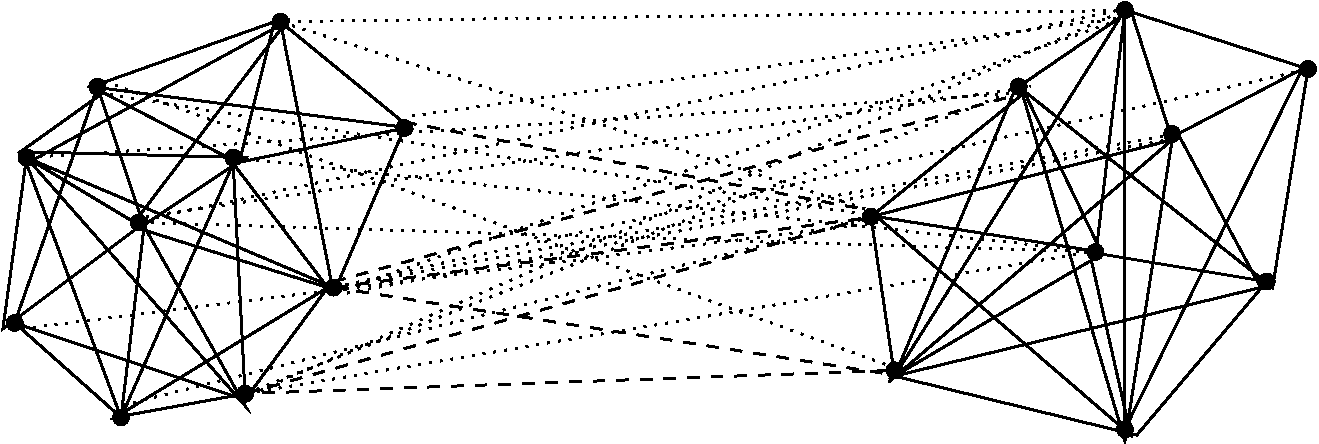
\includegraphics[width=0.4\linewidth]{Images/points_all}}
    \hspace{2cm}
    \subfigure[ With thresholding]{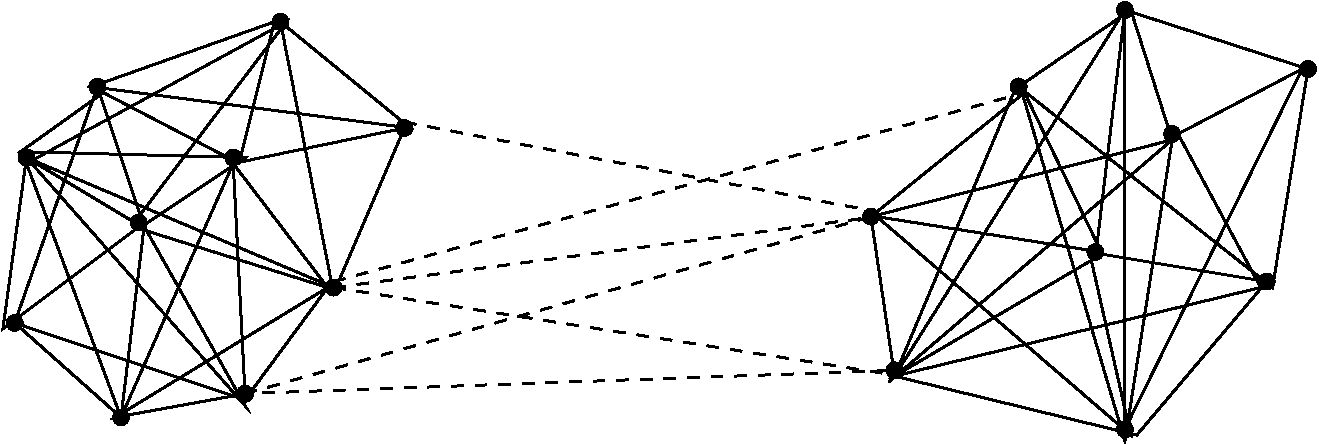
\includegraphics[width=0.4\linewidth]{Images/points_clusters_light}}
  \end{center}
  \caption{Thresholding of  the weighted adjacency graph.}
  \label{seuil}
 \end{figure}

From another point of view, the affinity matrix could be also interpreted as a
Gaussian weighted adjacency graph.
The thresholding will control the width of the neighborhoods. This parameter
chosen according to the affinity parameter  plays a similar role as the
parameter $\epsilon$ in case of the $\epsilon$-neighborhood graph. A
thresholding of the largest distances is equivalent to
cancel edges which connect data points very distant from each other as
represented in Figure \ref{seuil}. So it strengthens the affinity between
points among the same cluster and, so,  the separability between clusters.


\begin{figure}[!h]
  \begin{center}
      \subfigure[Clustering result with
      thresholding]{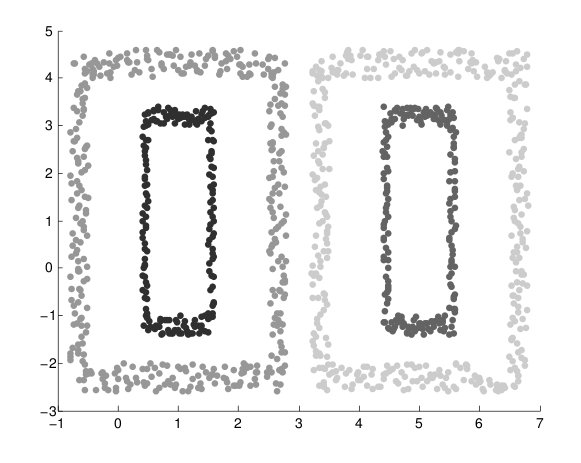
\includegraphics[width=0.45\linewidth]{Images/4rectAff}}
    \hspace{2cm}
    \subfigure[Affinity matrix : lower triangular without threshold, upper
    triangular with threshold]{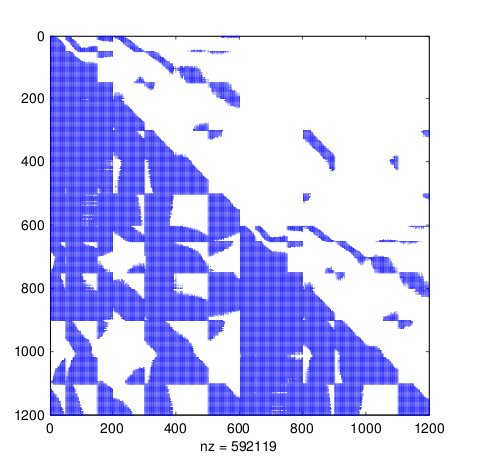
\includegraphics[width=0.35\linewidth]{Images/4rectAffSpars}}\\
    \subfigure[Memory cost function of the
    threshold]{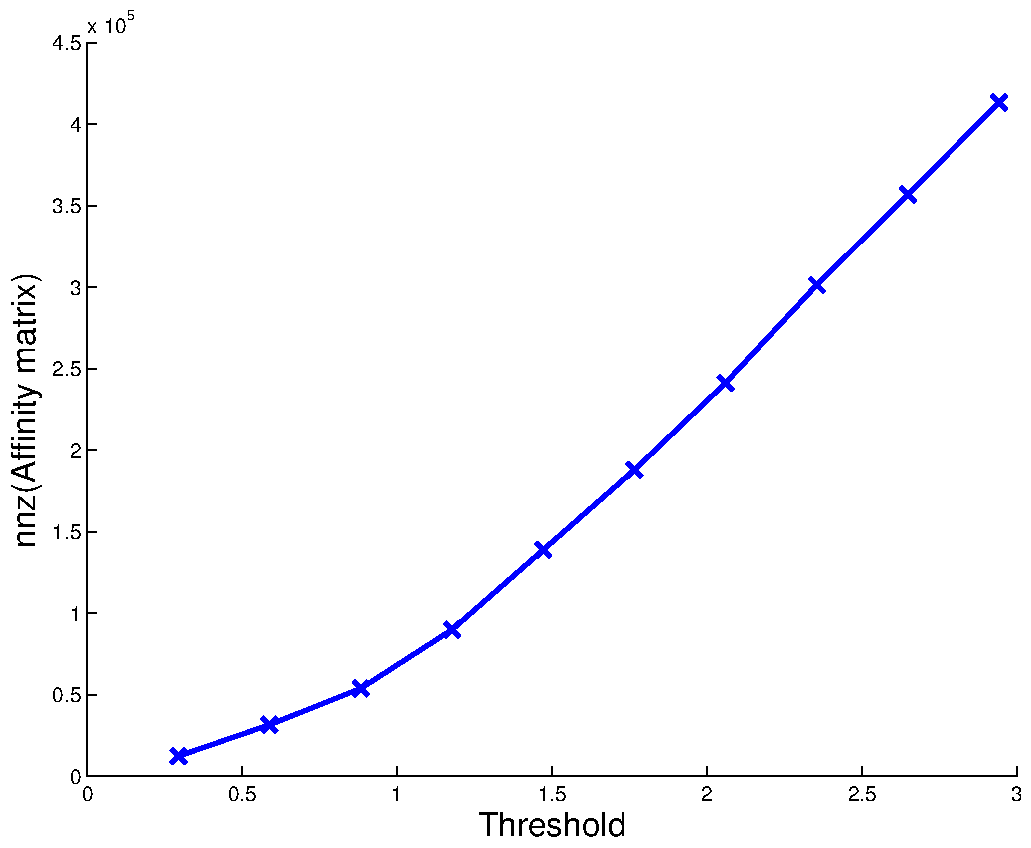
\includegraphics[width=0.4\linewidth]{Images/Memo4rect}}
    \hspace{2cm}
    \subfigure[Timings function of the
    threshold]{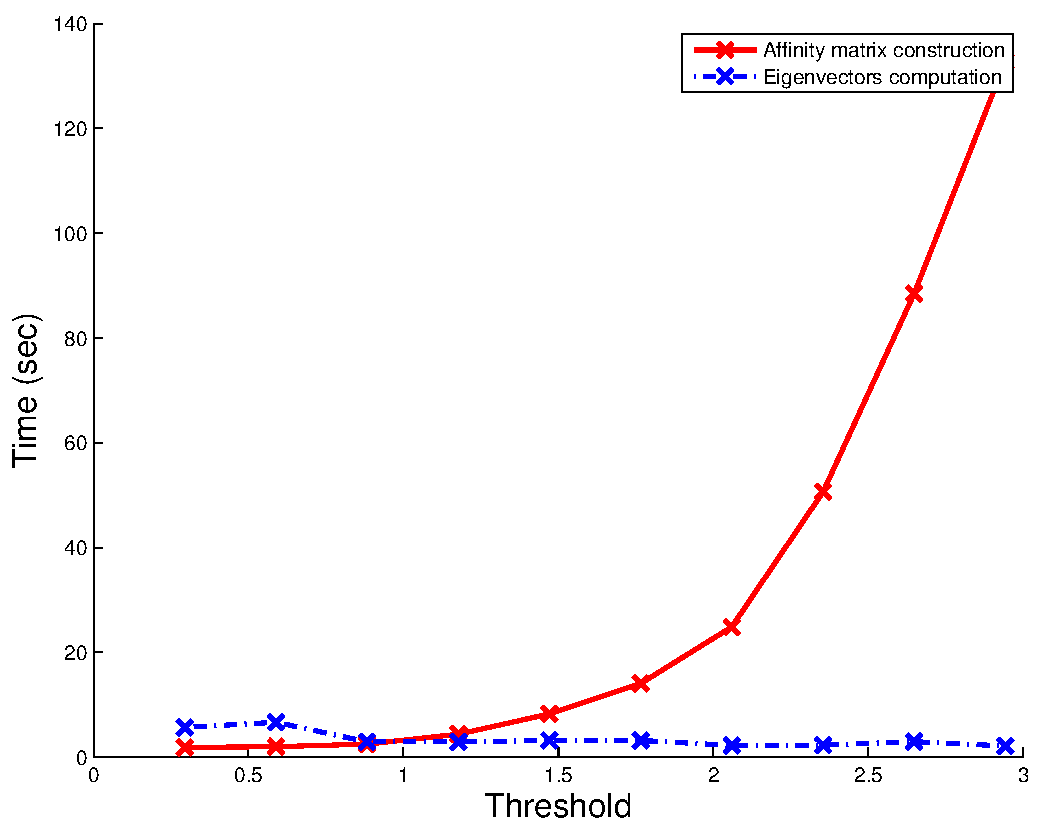
\includegraphics[width=0.4\linewidth]{Images/Timings4rect}}
  \end{center}
  \caption{Example 1: data set, sparsity of the affinity matrix, memory cost and timings}
  \label{4rect}
 \end{figure}


\subsection{Thresholding}
\label{threshold}

However a threshold should be heuristically defined to build an automatic sparsified matrix. We define the threshold that should represents a distance  adapted to any distribution of input data.  To do so, we start by defining a distance $D_{unif}$ as the distance in the case of the uniform distribution of $n$ points
in this enclosing p-th dimensional box in which the data are equidistant each other. This uniform distribution is reached
when dividing the box in $n$ smaller boxes all of the same size, each with
a volume of order $ D_{\max}^p / n$ where $D_{\max}$ is the maximum of the distance between two data point $x_i$ and $x_j$, $\forall i,j\in \{1,..,n\}$.
The corresponding edge size which defines $D_{unif}$ is given by:
\begin{equation}
D_{unif} = \frac{D_{\max}}{n^{\frac{1}{p}}} \, \label{factor}
 \end{equation}
The  thresholding will be function of $D_{unif}$ for any kind of data distribution $S$. 


\section{Numerical experiments}

As numerical experiments, we first begin by testing the thresholding on geometrical examples for  data set of small size. 
Then some tests on larger data set are investigated on image segmentation examples.


\subsection{First validations}
For first validations, we consider two geometrical examples represented in Fig.
\ref{4rect} (a) and Fig. \ref{cible} (a) in which the clusters could not be
separated by hyperplanes: the first one with four rectangles of $n=1200$ points 
and the second one with a target of $n=600$ points.
The eigenvectors were provided by the reverse communication required by the
Fortran library ARPACK \cite{lehoucq1998arpack}.

\begin{figure}[!h]
  \begin{center}
    \subfigure[Clustering result with
    thresholding]{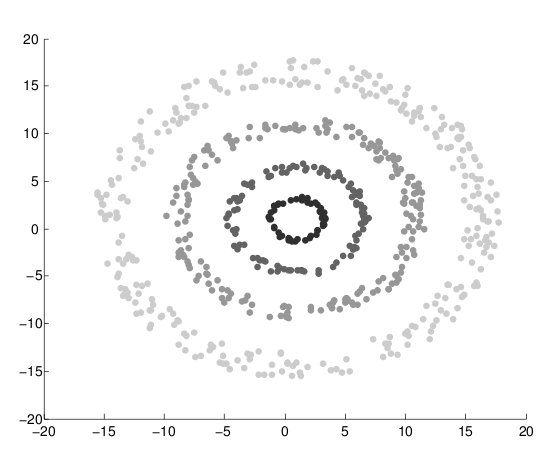
\includegraphics[width=0.45\linewidth]{Images/cibleclust}}
    \hspace{2cm}
    \subfigure[ Affinity matrix : lower triangular without threshold, upper
    triangular with threshold]{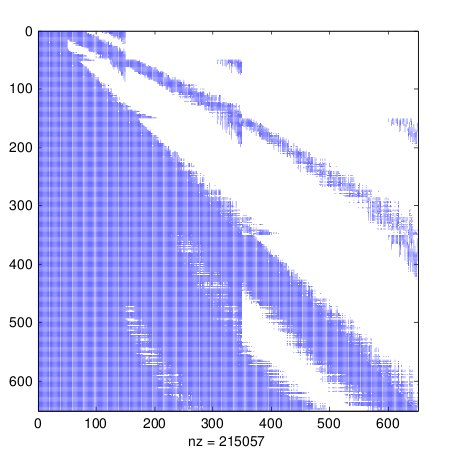
\includegraphics[width=0.34\linewidth]{Images/CibleAffSpars}}\\
    \subfigure[Memory cost function of the
    threshold]{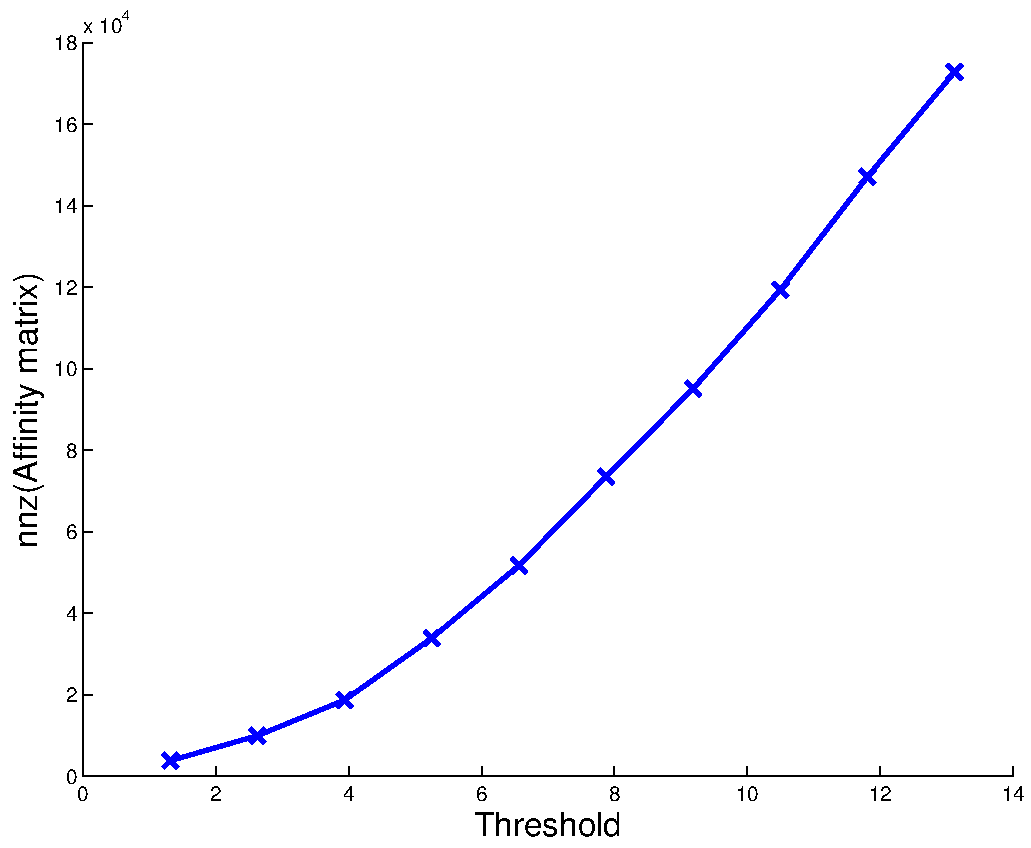
\includegraphics[width=0.4\linewidth]{Images/MemoCible}}
    \hspace{2cm}
    \subfigure[Timings function of the
    threshold]{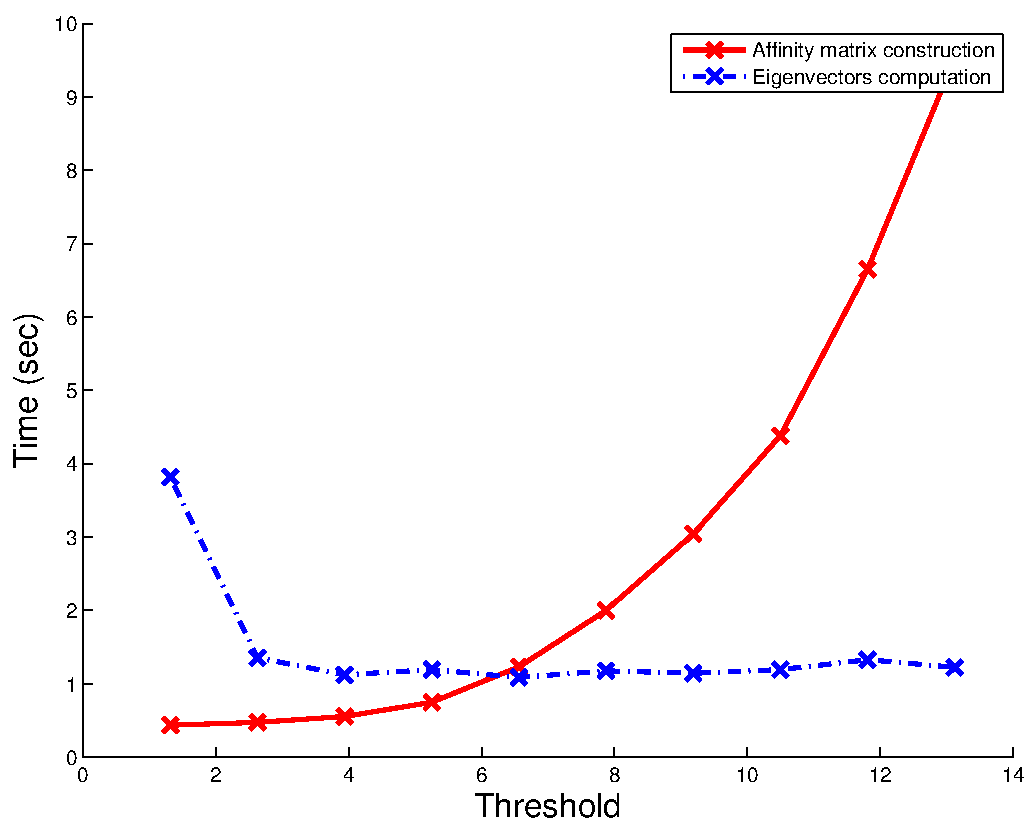
\includegraphics[width=0.4\linewidth]{Images/TimingsCible}}
  \end{center}
  \caption{Example 2: data set, sparsity of the affinity matrix, memory cost and timings}
  \label{cible}
 \end{figure}


We measure the timings in seconds, in function of the threshold, of the
construction of the affinity matrix and of the computation of eigenvectors.
The memory cost is evaluated in function of the threshold by the number of
non-zeros elements in the affinity matrix.

We can notice on (c) sub-figure that we gain a lot of memory when we decrease
the threshold i.e.  when we drop the connections of points at a distance larger
than it. In fact, this sub-figure shows the memory space required for the storage of the affinity matrix by using a sparse structure $(i,j,value(A_{ij}))$.

We also remark on (d) sub-figure that the time to construct the affinity matrix decreases in
this case. Indeed, the computation of the component $A_{ij}$ requires to
compute an exponential (\ref{defaff}). So because the selection of the connections
we keep is done only with the distance, we don't compute the non-useful
components and save a lot of floating point operations.

So we have a response to the memory consumption and timing limitations we
mentioned previously. As we can see on the first validations, a thresholding strategy allows for considerable gains in terms of memory requirements and computational performance.

If we look the timing for the extraction of the eigenvectors, the time
remains the same for acceptable values of the threshold.
But we encounter a limit to the sparsification technique with example 2: a
strong threshold could imply a very sparsified affinity matrix and an ill-conditioned matrix. 
In this case, the eigenvector computation becomes the most time consuming
task in the sense that the algorithm from Arnoldi method does not converge.


\subsection{Another application: image segmentation} \label{image}

For image segmentation, the domain decomposition is applied geometrically on the image and also on the brightness distribution (or color levels) as shown in the figure \ref{ExampleImage}. In fact, we include both 2D geometrical information and 1D 
brightness (or 3D color levels) information in the spectral clustering method
in the sense that there does not exist some privileged directions with very
different magnitudes in the distances between points along theses directions.
The step between pixels and brightness (or color levels) are about the same
magnitude.
Thus, a new distance in the affinity measure is defined for image. In the same
way, a global heuristic for the Gaussian affinity parameter is proposed in
which both dimension of the problem as  well as the density of points in the
given 3D (or 5D for colored image) are integrated.  By considering the size of
the image $I$, the Gaussian affinity $A_{ir}$ is defined as follows:
\begin{equation}
A_{ir}=\begin{cases}
\exp\left(-\frac{d\left(I_{ij},I_{rs}\right)^2}{(\sigma/2)^2}\right) \text{\  if $(ij)\neq (rs)$,}\\ 
0 \ \text{otherwise,} \nonumber
\end{cases}
\end{equation}
with the distance between the pixel $(ij)$ and $(rs)$ defined by:
\begin{equation}
d\left(I_{ij},I_{rs}\right)=\sqrt{\left(\frac{i-r}{l}\right)^2+\left(\frac{j-s}{m}\right)^2+\left(\frac{I_{ij}-I_{rs}}{256}\right)^2}
\label{puceaff}
\end{equation}

\begin{figure}[!h]
  \begin{center}
  {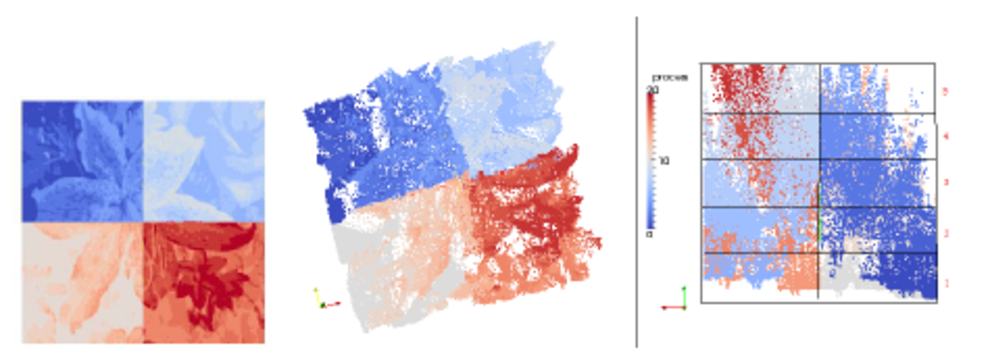
\includegraphics[width=1\linewidth]{Images/decoupimage}}
  \end{center}
  \caption{Example of domain decomposition for image segmentation : geometrical decomposition on the left, brightness distribution and decomposition on the right.}
  \label{ExampleImage}
 \end{figure}


Parallel spectral clustering was used for image segmentation \cite{mouysset3}
and we present now the first results of the sparsified parallel spectral
clustering applied on image segmentation.

\subsubsection{Computational environment}

\

The parallel numerical experiments were carried out on the Hyperion
supercomputer\footnote{http://www.calmip.cict.fr/spip/spip.php?rubrique90}.
Hyperion is the latest supercomputer of the CICT (Centre Interuniversitaire de
Calcul de Toulouse). With its 352 bi-Intel "Nehalem" EP quad-core nodes it can
develop a peak of 33TFlops. Each node has 4.5 GB memory dedicated for each of
the cores and an overall of 32 GB fully available memory on the node that is
shared between the cores.

\subsubsection{3D image segmentation}

\

The first example is a Mahua illustration of Benjamin Zhang Bin which presents some continuous degradation of grayscale levels.
This grayscale image of $232764$ data points is divided in 20 subdomains.
We perform experiments with different values of the factor. The threshold is given by the product of the factor with $D_{unif}$  defined by (\ref{factor}).
Fig. \ref{statBenji} summarizes the memory consumption
(maximum consumption on one sub-domain, average consumption on all subdomains,
minimum consumption on one subdomain).

\begin{figure}[!h]
  \begin{center}
  {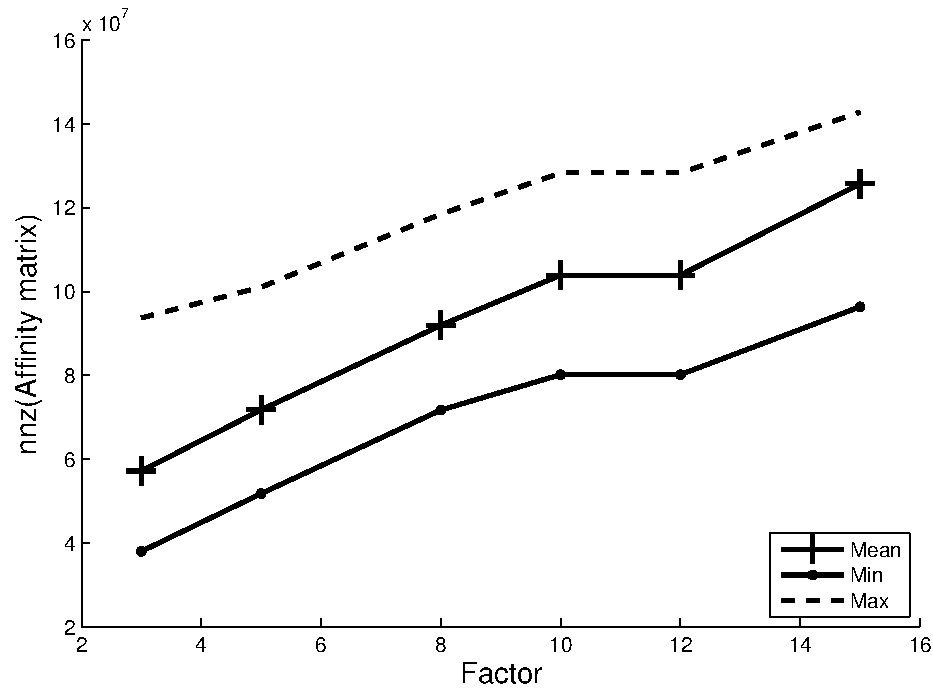
\includegraphics[width=0.65\linewidth]{Images/BenjaminStat2}}
  \end{center}
  \caption{Example of image segmentation in grayscale: memory cost function of the factor}
  \label{statBenji}
 \end{figure}

As we can observe, we are able to decrease this memory consumption by a
factor two on average without losing the quality of image segmentation as we
can see in Fig. \ref{benji}. There is no significant difference
between the result with the full matrix and the one with sparsification with a
factor 3.

\begin{figure}[!h]
  \begin{center}
  \begin{center}
  \subfigure[original]{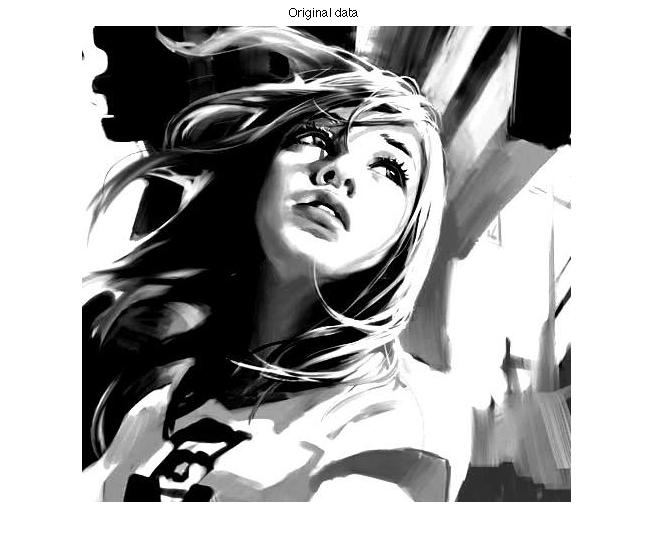
\includegraphics[width=0.40\linewidth]{Images/BenjiOriginal}}
  \subfigure[full]{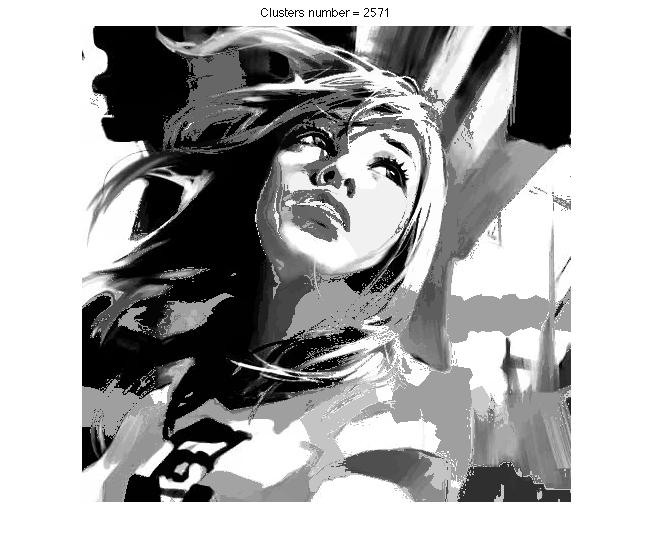
\includegraphics[width=0.40\linewidth]{Images/BenjiFull}}\\
  \subfigure[factor=3]{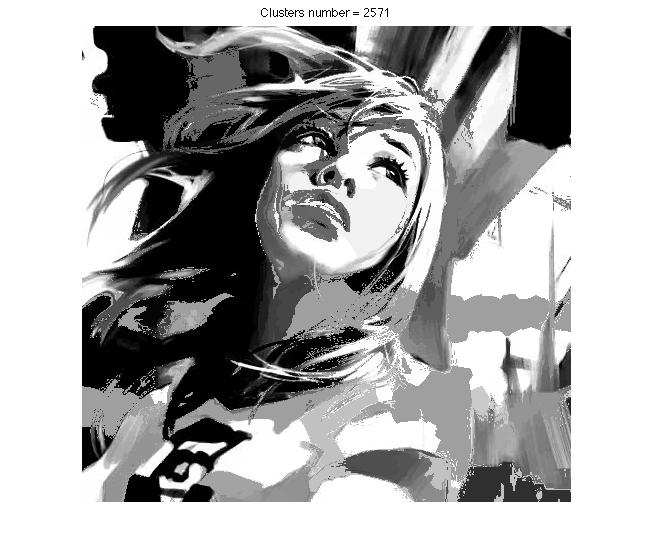
\includegraphics[width=0.40\linewidth]{Images/BenjiSparse3}}
  \end{center}
  \end{center}
  \caption{Example of 3D image segmentation: original data set, clustering result
  without thresholding and with thresholding (factor 3)}
  \label{benji}
 \end{figure}

\subsubsection{5D image segmentation}

\

The second example represents a photo of Yann Arthus Bertrand of colored fields in Vaucluse. %This picture has a geometrical colored segmentation. 
This is  a color image of 128612 points which is also divided in 20 subdomains. In Fig. \ref{stat}, the memory
consumption is plotted.

With this example we are able to divide by 10 this consumption when we take a
factor of 1 without loss of quality as we can see in Fig. \ref{arthus2}.

\begin{figure}[!h]
  \begin{center}
  {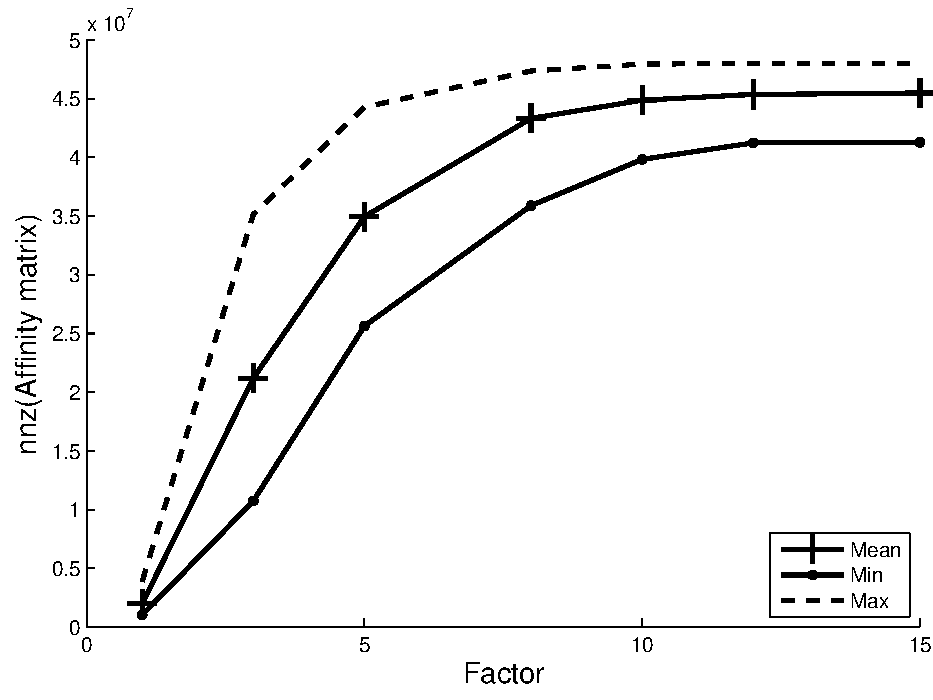
\includegraphics[width=0.65\linewidth]{Images/Arthus2Stat2}}
  \end{center}
  \caption{Example of 5D image segmentation in colors: memory cost function of the factor}
  \label{stat}
 \end{figure}

\begin{figure}[!h]
  \begin{center}
  \subfigure[original]{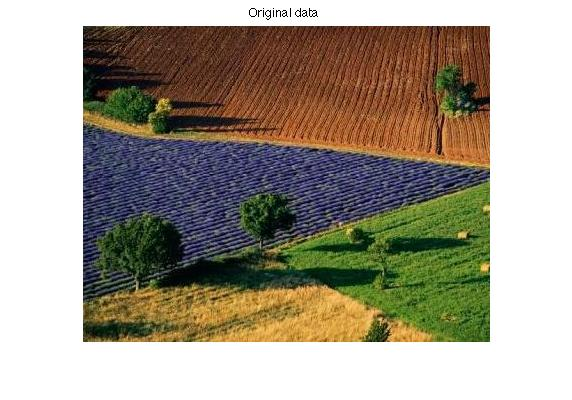
\includegraphics[width=0.49\linewidth]{Images/Arthus2original}}
  \subfigure[full]{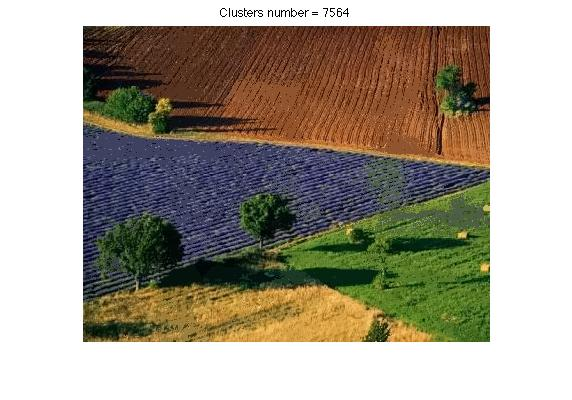
\includegraphics[width=0.49\linewidth]{Images/Arthus2full}}\\
  \subfigure[factor=1]{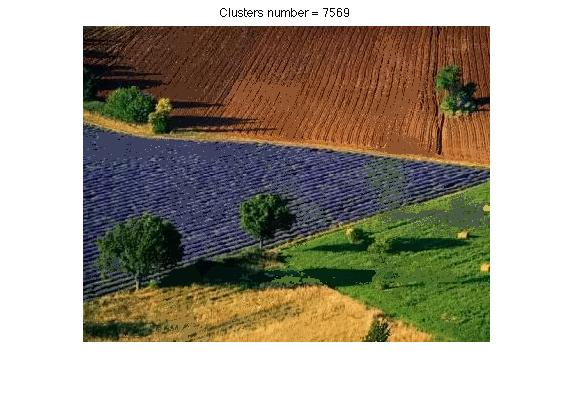
\includegraphics[width=0.49\linewidth]{Images/Arthus2S1}}
  \subfigure[factor=0.9]{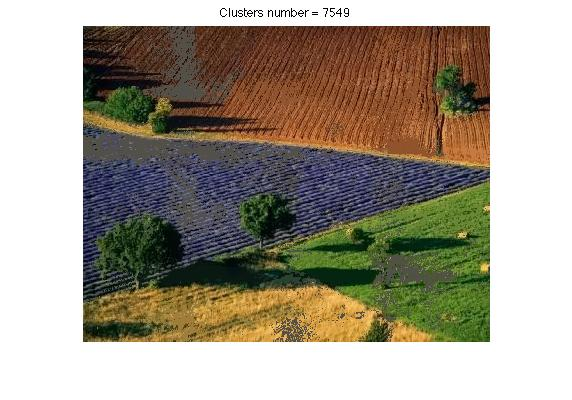
\includegraphics[width=0.49\linewidth]{Images/Arthus2S09}}\\
  \end{center}
  \caption{Example of image segmentation: original data set, clustering result
  without and with thresholding (factor = 1 and factor = 0.9)}
  \label{arthus2}
 \end{figure}

%\pagebreak[4]
However with this example, we tried to further reduce the factor. We
experiment that with the value 1, we reach a limit because with factors lower
than~1 we notice a significant loss of quality in the segmentation as we can
see in subfigure (d) of Fig. \ref{arthus2} that presents the results with a factor of $0.9$. As $D_{unif}$ defined by (\ref{factor}) represents the distance for an uniform distribution, clusters may exist if there are data points which are separated by a fraction of $D_{unif}$. So for a value of factor lower than 1, 
the thresholding could affect the clustering result. 

\section{Conclusion and ongoing works}

As we mentioned in the conclusion of our work at the previous VECPAR
conference \cite{mouysset3}, we have begun to study sparsification techniques in the
construction of affinity matrix by dropping some components that correspond to
points at a distance larger than a threshold. A threshold based on uniform distance was defined for any kind of data distribution. 
This distance could be considered as a limit threshold to preserve the clustering results.
We validate this approach in matlab by showing that the number of non zero of the
affinity matrix decreases with still some good results in terms of spectral
clustering and even some gains in the time spent to compute the affinity
matrix.

These results are confirmed when we use sparsification with our parallel
spectral clustering solver. We can show that we are able to reduce
significantly the size of the affinity matrix without loosing the quality of
the segmentation solution.

We have still more experiments to perform and some improvements to achieve.
First, we have to investigate in all the available tunings in ARPACK 
to be sure to use the less memory when computing the eigenvectors and
eigenvalues. We will then be able to compare the timings with or without
sparsification. And finally, we
have to perform experiments with bigger images for which we can't have
solution if we don't use sparsification.

\begin{thebibliography}{5}
%
\bibitem{speC}
Ng, A. Y., Jordan, M. I.  and Weiss, Y.
On spectral clustering: analysis and an algorithm.
\emph{Proc.Adv.Neural Info.Processing Systems}, 2002.

%\bibitem{diffus}
%  Diffusion Maps, Spectral Clustering and Eigenfunctions of Fokker-Planck operators.
%  Nadler, B. and Lafon, S. and Coifman, R.R. and Kevrekidis, I.G.
%  \emph{Arxiv preprint math.NA/0506090}, 2005.

\bibitem{Chen10}
Chen, W-Y., Yangqiu, S., Bai H., Lin C-J. and Chang E. Y.
Parallel Spectral Clustering in Distributed Systems.
\emph{IEEE Transactions on Pattern Analysis and Machine Intelligence},2010.


%\bibitem{eigen}
%Belkin, M.  and Niyogi, P.
%Laplacian Eigenmaps and Spectral Techniques for Embedding and Clustering.
%\emph{Advances in Neural Information Processing Systems}, 2002.
%
%\bibitem{mouysset}
%Mouysset, S. and Noailles, J. and Ruiz, D.
%Using a Global Parameter for Gaussian Affinity Matrices in Spectral Clustering,
%  \emph{High Performance Computing for Computational Science: 8th International Conference}, 2008.



\bibitem{song}
Song, Y. and Chen, W.Y. and Bai, H. and Lin, C.J. and Chang, E.Y.
Parallel spectral clustering,
\emph{Processing of European Conference on Machine Learning and Principles and Practice of Knowledge Discovery in Databases}, 2008.

\bibitem{fowlkes}
  Fowlkes, C. and Belongie, S. and Chung, F. and Malik, J.,
  Spectral grouping using the Nystrom method,
\emph{IEEE Transactions on Pattern Analysis and Machine Intelligence}, 2004.

\bibitem{yan2009fast}
Yan, D. and Huang, L. and Jordan, M.I.
Fast approximate spectral clustering,
\emph{Proceedings of the 15th ACM SIGKDD international conference on Knowledge discovery and data mining},2009.



\bibitem{mouysset3}
Mouysset, S. and Noailles, J., Ruiz, D. and Guivarch, R..
On a strategy for Spectral Clustering with parallel computation,
\emph{High Performance Computing for Computational Science: 9th International Conference}, 2010.


\bibitem{anderson1999lapack}
Anderson, E. and Bai, Z. and Bischof, C. and Blackford, S. and Demmel, J. and Dongarra, J. and Du Croz, J. and Greenbaum, A. and Hammarling, S. and McKenney, A. and others
LAPACK Users' guide,
 \emph{Society for Industrial Mathematics}, 1999.


\bibitem{mouysset2}
Mouysset, S. and Noailles, J. and Ruiz, D.
On an interpretation of Spectral Clustering via Heat equation and Finite Elements theory,
\emph{International Conference on Data Mining and Knowledge Engineering}, 2010.



\bibitem{lehoucq1998arpack}
Lehoucq, R.B. and Sorensen, D.C. and Yang, C.,
 ARPACK users' guide: solution of large-scale eigenvalue problems with implicitly restarted Arnoldi methods,
\emph{SIAM},1998. 





%
\end{thebibliography}





\end{document}
